\chapter{Study Background} 
\label{sec:background}

In this chapter we contextualize our work, giving an overview of code smells and machine learning, the base concepts used in this study.

\section{Code Smell}

Code anomaly, so-called "code smell", is an implementation choice that indicates a design problem which violates the well-known principles of cohesion, abstraction and separation of concerns \cite{oizumi2016code} on software development. There are more than 20 \cite{fowler1999refactoring} different types of code smells that contributes to increase comprehension effort \cite{abbes2011empirical} and leads to design degradation \cite{oizumi2016code}. The adoption of refactoring, a clean-up process that improves the code's internal structure \cite{fowler1999refactoring}, is the way out to prevent the presence of code smells in code. Fowler et. al. \cite{fowler1999refactoring} about 20 sets of symptoms of code smells. These include large classes, feature envy, long parameter lists, and lazy classes. Each code-smell type is accompanied by refactoring suggestions to remove it.

We chose four different types of code smells to carry out experiments, which are detailed in Section \ref{sec:codeSmellTypes}.

%\subsection{Software metrics}

\section{Machine Learning}
\cite{vanderplas2016python} states that Machine learning involves building mathematical models to help
understand data. Once these models have been fit to previously
seen data, they can be used to predict and understand aspects of newly observed data. The learning process might be categorized into two main types: supervised learning and unsupervised learning. 

\section{Supervised and Unsupervised Learning}

Supervised learning is a method that attempts to discover the relationship between input attributes (independent variables) and a target attribute (referred to as a dependent variable).
The relationship that is discovered is represented in a structure referred
to as a Model. Models describe and explain phenomena which are
hidden in the dataset and which can be used for predicting the value of
the target attribute whenever the values of the input attributes are known.
The supervised methods can be implemented in a variety of domains such
as marketing, finance and manufacturing  \cite{rokach2008data}. 

Unsupervised learning involves modeling the features of a dataset without reference to any label. These models include tasks such as clustering, in which data is automatically assigned to some number of discrete groups. As a result, the model can infer labels on unlabeled data \cite{vanderplas2016python}.

\section{Decision Tree Classifier}

A decision tree is a type of supervised learning that uses a tree structure to represent a number of possible decision paths and
an outcome for each path. They’re very easy to understand and
interpret, and the process by which they reach a prediction is completely transparent \cite{grus2019data}. Due to its transparency, this technique is frequently
used in applied fields such as finance, marketing, engineering and medicine \cite{rokach2008data}. For having this self-explanatory feature, there is
no need to be a data mining expert in order to follow a certain decision
tree. \cite{rokach2008data}

Decision trees can easily handle a mix of
numeric and categorical attributes and
can even classify data for which attributes are missing \cite{grus2019data}.
When a decision tree is used for classification tasks  (which produce categorical
outputs), it is most commonly referred to as a classification tree. When it is used for regression tasks, it is
called a regression tree  (which produce numeric outputs) \cite{rokach2008data}. The Figure \ref{fig:exampleDecisionTreeGuessAnimal} shows a typical decision tree classifier, an example that predicts an animal, based on a set of characteristics. Instances are classified by navigating them from the root of the tree
down to a leaf according to the outcome of the tests along the path. 

\begin{figure}[ht]
\centering
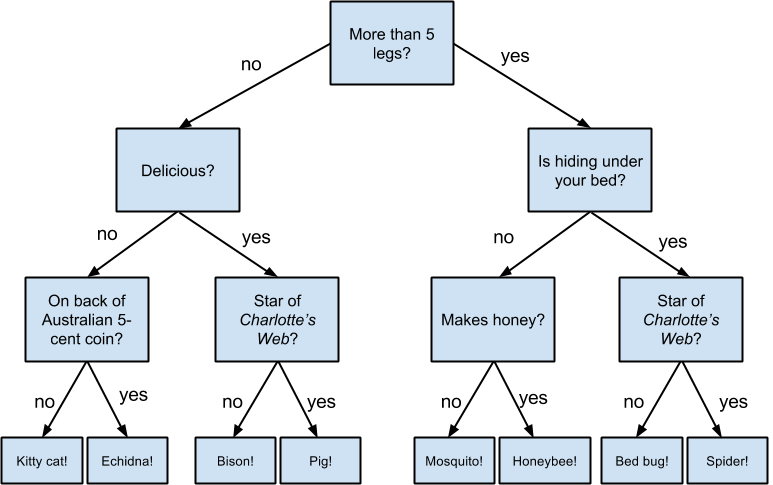
\includegraphics[width=400px]{figures/decision_tree_example.png}
\caption{Example: A decision tree to guess an animal. \cite{grus2019data}}
\label{fig:exampleDecisionTreeGuessAnimal}
\end{figure}

As seen in Figure \ref{fig:exampleDecisionTreeGuessAnimal}, the decision tree consists of a node called a “root” that has no incoming edges. All other nodes have exactly one incoming edge. A node
with outgoing edges is referred to as an “internal” node or a “test” node.
All other nodes are called “leaves”. In a decision tree, each internal node splits the instance
space into two or more sub-spaces according to a certain discrete function
of the input attributes values. In the simplest and most frequent case, each
test considers a single attribute, such that the instance space is partitioned
according to the attributes value. In the case of numeric attributes, the
condition refers to a range. Each leaf is assigned to one class representing the most appropriate
target value \cite{rokach2008data}.

To comprehend any predictions, we start with a root of a tree; we consider the characteristic that corresponds to the root and we define to which branch the observed value of the given characteristic corresponds. Then, we consider the node in which the given
branch appears. We repeat the same operations for this node until we reach a leaf \cite{rokach2008data}.

Algorithms for constructing decision trees work top-down, by choosing a feature at each step that best splits the set of instances \cite{rokach2008data}. Different algorithms use different metrics for measuring the "best",  generally measuring the homogeneity of the target feature within the subsets. So these metrics are applied to each candidate subset, and the resulting values are combined to provide a measure of the quality (or impurity) of the split. There are two well known splitting criteria which can be cited:

\textbf{Information Gain.} is an impurity-based criteria that uses the entropy measure as the impurity measure \cite{rokach2008data}. Entropy is defined as:
\begin{equation}
Gini(T)= - \sum_{i=1}^{J}p_{i}\log_{2}p_{i}
\end{equation}

where $p_{1},p_{2},...$ are fractions of samples and represent the percentage of each class present in the child node that results from a split in the tree. Thus, the Information gain is the degree of impurity among  parent and children:

\begin{equation}
\overbrace{IG(T,a)}^{Information \ Gain} = \overbrace{H(T)}^{Entropy \ (parent)} - \overbrace{H(T|a)}^{Weighted \ sun \ of \ Entropy \ (Children)}
\end{equation}

\textbf{Gini Index.} Is an impurity-based criteria that measures the divergences
between the probability distributions of the target attributes \cite{rokach2008data} values and is defined as:

\begin{equation}
Gini(p) = 1 - \sum_{i=1}^{J}{p_{i}}^2
\end{equation}

where  $i \in \{1,2,...,J\}$ and $p_{i}$ the fraction of items labeled with class $i$ in the set.